\documentclass[a4paper,9pt]{extarticle}

%=========================================================
% PACKAGES
%=========================================================

\usepackage[
a4paper,
top=1.8cm,
bottom=1.5cm,
footskip=7mm,
left=1cm,
right=1cm,
headheight=14pt,
headsep=5mm
]{geometry}
\usepackage[T1]{fontenc}
\usepackage[utf8]{inputenc}
\usepackage[french]{babel}

\usepackage[sfdefault]{FiraSans}
\renewcommand{\familydefault}{\sfdefault}

\usepackage{multicol}
\setlength{\columnsep}{0.7cm}

\usepackage{amsmath,amssymb}

\usepackage{titlesec}
\usepackage{enumitem}

\usepackage{tcolorbox}
\tcbuselibrary{skins,breakable}

\usepackage{xcolor}

\usepackage{graphicx}
\usepackage{float}

\usepackage{tikz}

\usepackage{fancyhdr}
\usepackage[hidelinks]{hyperref}


%=========================================================
% PAGE SETTINGS
%=========================================================

\setlength{\parindent}{0pt}
\setlength{\parskip}{1.5pt}

\setlength{\abovedisplayskip}{4pt}
\setlength{\belowdisplayskip}{4pt}

\setlist[itemize]{
leftmargin=*,
itemsep=1pt,
topsep=1pt
}


%=========================================================
% COLORS
%=========================================================

\definecolor{Blue}{HTML}{E3F0FF}
\definecolor{Green}{HTML}{E3F7EA}
\definecolor{Pink}{HTML}{FFE5ED}
\definecolor{Orange}{HTML}{FFF0DC}
\definecolor{Purple}{HTML}{EEE7FF}
\definecolor{Yellow}{HTML}{FFFADB}


\definecolor{BlueTitle}{HTML}{285B8F}
\definecolor{GreenTitle}{HTML}{287052}
\definecolor{PinkTitle}{HTML}{A84063}
\definecolor{OrangeTitle}{HTML}{A96500}
\definecolor{PurpleTitle}{HTML}{6245A5}


%=========================================================
% HEADER
%=========================================================

\pagestyle{fancy}

\fancyhf{}

\fancyhead[L]{\small\textbf{Game Theory and Strategic Decisions}}
\fancyhead[C]{\small Braess Paradox, Bayesian Games, Conditional Probability}
\fancyhead[R]{\small Week 05 --- 05-11/10/2026}

\fancyfoot[C]{\small\href{https://github.com/AlphaXT38G/notes_ba5}{github.com/AlphaXT38G/notes\_ba5}}
\fancyfoot[R]{\small \thepage}

\renewcommand{\headrulewidth}{0.4pt}



%=========================================================
% TITLES
%=========================================================

\titleformat{\section}
{\large\bfseries\color{BlueTitle}}
{}{0pt}{}

\titlespacing{\section}
{0pt}{6pt}{3pt}


% separator

\newcommand{\separator}{
\vspace{2pt}
\hrule
\vspace{3pt}
}


%=========================================================
% BOXES
%=========================================================

% Boxes are kept whole (unbreakable): inside multicols, a box split by tcolorbox
% leaves an empty column behind it.

% DEFINITION - blue
\newtcolorbox{definition}{
enhanced,
unbreakable,
colback=Blue,
colframe=BlueTitle,
boxrule=0.7pt,
arc=0mm,
title=\textbf{Definition},
fonttitle=\bfseries
}

% IMPORTANT - pink
\newtcolorbox{important}{
enhanced,
unbreakable,
colback=Pink,
colframe=PinkTitle,
boxrule=0.7pt,
arc=0mm,
title=\textbf{Key idea},
fonttitle=\bfseries
}

% FORMULAS - green
\newtcolorbox{formula}{
enhanced,
unbreakable,
colback=Green,
colframe=GreenTitle,
boxrule=0.7pt,
arc=0mm,
title=\textbf{Key formulas},
fonttitle=\bfseries
}

% WARNING - orange
\newtcolorbox{warning}{
enhanced,
unbreakable,
colback=Orange,
colframe=OrangeTitle,
boxrule=0.7pt,
arc=0mm,
title=\textbf{Warning},
fonttitle=\bfseries
}

% EXAMPLE - purple
\newtcolorbox{example}{
enhanced,
unbreakable,
colback=Purple,
colframe=PurpleTitle,
boxrule=0.7pt,
arc=0mm,
title=\textbf{Example},
fonttitle=\bfseries
}

% SUMMARY - orange
\newtcolorbox{summary}{
enhanced,
unbreakable,
colback=Yellow,
colframe=OrangeTitle,
boxrule=0.7pt,
arc=0mm,
title=\textbf{Summary},
fonttitle=\bfseries
}



%=========================================================
% FIGURE BOX
%=========================================================

\newtcolorbox{figurebox}{
enhanced,
colback=white,
colframe=gray,
boxrule=0.5pt,
arc=0mm,
center
}



%=========================================================
% DOCUMENT
%=========================================================

\begin{document}

%\footnotesize   --> To reduce the size of the text

\thispagestyle{fancy}



\begin{multicols}{2}



%=========================================================
\section{Today's Agenda}


\begin{itemize}

\item Game theory real world paradoxes: the \textbf{Braess paradox}.

\item Back to simultaneous-move games of incomplete information: the \textbf{free riding
game}.

\item In preparation to next lecture: \textbf{conditional (Bayesian) probability} with
examples.

\end{itemize}


%=========================================================
\section{The Braess Paradox}


\begin{definition}

\textbf{BRAESS PARADOX}

$N$-player, simultaneous-move game (complete information) modeling a transportation network.

Paradox: \textbf{adding a new, very fast route to a transportation network can increase
traffic and transportation time for everybody}.

\end{definition}


\begin{example}

\textbf{Real-world cases}

\begin{itemize}

\item \textbf{Stuttgart, 1969}: shortly after D.\ Braess published his theory, the city
invested heavily in its downtown road network by building a highly efficient new road
segment. Traffic immediately ground to a halt. When the city closed the newly built road
section, traffic immediately returned to normal.

\item \textbf{NYC, 1990}: 42nd street (one of Manhattan's busiest crosstown arteries) closed
on ``Earth day''. Media outlets warned of a ``traffic apocalypse'', but when the street
closed, the surrounding gridlock dropped drastically, and traffic moved faster.

\item \textbf{Seoul, South Korea, 2003}: the destruction of a six-lane highway to build a
park actually improved travel time into and out of the city. Traffic volume stayed roughly
the same before and after.

\end{itemize}

\end{example}



%=========================================================
\section{Braess -- Initial Situation}


\begin{center}

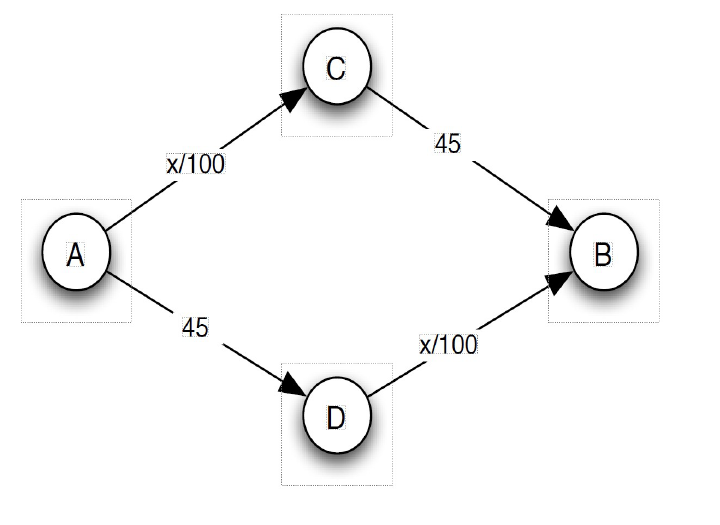
\includegraphics[
width=0.7\linewidth
]{../images/week05_01.png}

\end{center}


\begin{itemize}

\item \textbf{N = 4000 cars} (players). Two \textbf{directed} routes to go from A to B.

\item Travel time on an ``edge'' of the graph (e.g.\ edge AC) is a function of the number of
cars: $T_e = T_e(x)$.

\item Payout for each car is $-T_e(x)$: each car's objective is to \textbf{minimize} travel
time.

\end{itemize}


\textbf{Is there a NE in which all cars take the same route?} No. If all cars went through C
(route AC+CB), travel time would be $4000/100 + 45 = 85$ minutes. A car would have an
incentive to switch to the route through D (AD+DB): $1/100 + 45 = 45.01$.


\begin{important}

For different cars to take different routes (still a \textbf{pure-strategy NE}), since all
cars are identical, with the same payout, travel time should be the same on the two routes
\emph{in the limit $N \to \infty$, in which a single car cannot affect the travel time of a
route}.

\textbf{2000 cars on each route is a NE}, with travel time $2000/100 + 45 = 65$ minutes for
each car.

\end{important}


\begin{example}

\textbf{Odd number of cars}: e.g.\ 7 cars, 3 on AC+CB and 4 on AD+DB. Is this a NE? Yes,
because even for the cars on AD+DB, switching to AC+CB would leave travel time unchanged.

\end{example}



\end{multicols}


\end{document}
